\newpage
\subsection{Applicazione}
In questi scenari faremo largo uso della libreria\termine{vue.js} per aggiornare le visualizzazioni, all'interno della chat, delle bolle lista modificate. Lo schema di attivazione è abbastanza semplice in quanto una volta passati al presenter della bolla lista i dati modificati, la libreria \termine {vue.js} si occuperà del aggiornamento in tutte le chat che dipendono dalla lista modificata.
\subsubsection{Creazione di una lista}

\label{Creazione di una lista}
\begin{figure}[H]
	\centering
	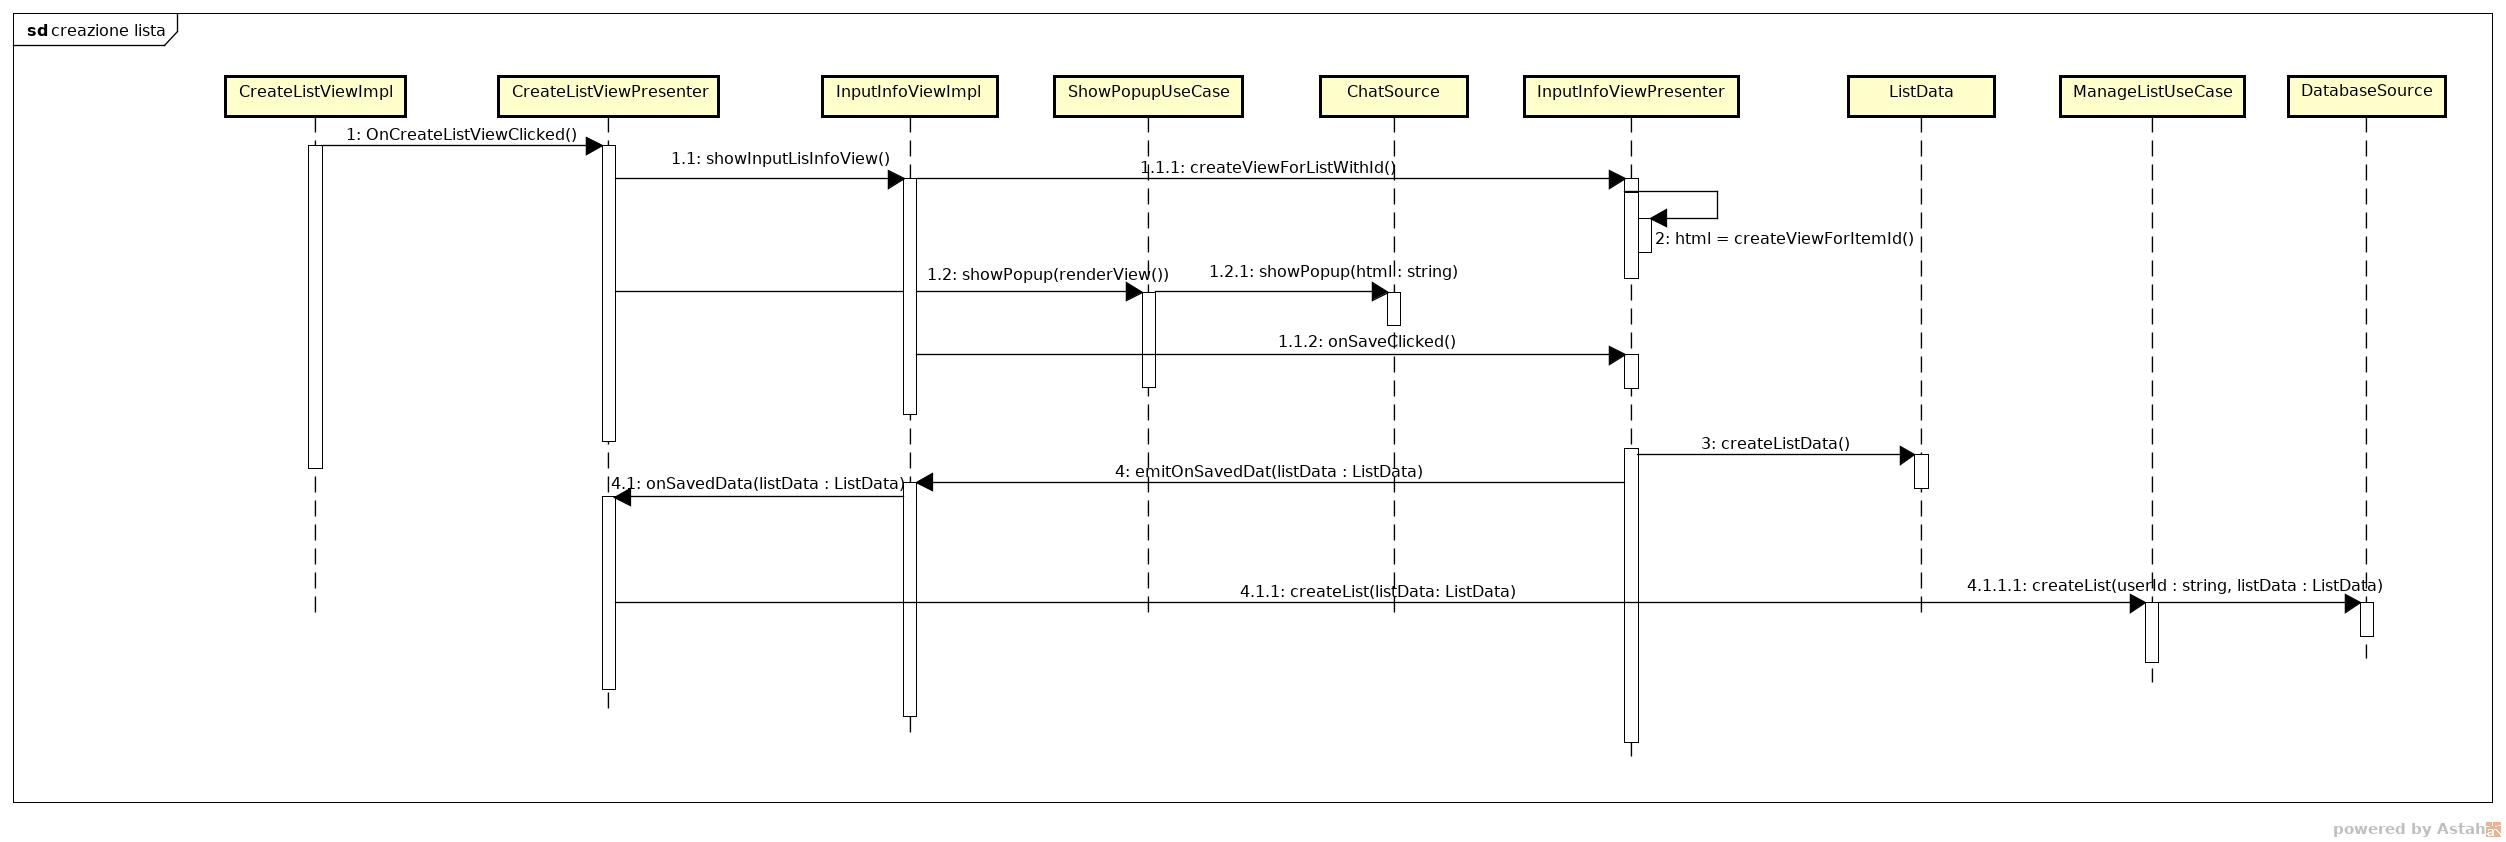
\includegraphics[ width=\textwidth]{Sezioni/Diagrammi/img_app/creazione_lista.jpg}
	\caption{Creazione di una lista}
\end{figure}

Questo scenario rappresenta l'utente che vuole creare una nuova lista nella chat di \termine{rocket.chat}. Inanzitutto alla pressione del pulsante creazione lista verrà emesso un evento che verrà catturato dalla classe \textit{CreateListVIewImpl} che demanderà la gestione di esso al presenter. Quest'ultimo attraverso il metodo \textit{showInputListInfoView} recupererà il codice html relativo al inserimento dei dati per la creazione della lista e lo mostrerà al utente attraverso un popup creato appositamente dalla chat. Dopo aver finito di inerire i dati desiderati l'utente premerà il relativo pulsante di salvataggio. In questo modo verrà emesso l'evento di salvataggio che verrà gestito dal presenter di \textit{showInputListInfoView} e infine attraverso il metodo \textit{createList} la lista verrà creata nel \termine{database} insieme al id del creatore .



\subsubsection{Cancellazione di una lista}

\label{Cancellazione di una lista}
\begin{figure}[H]
	\centering
	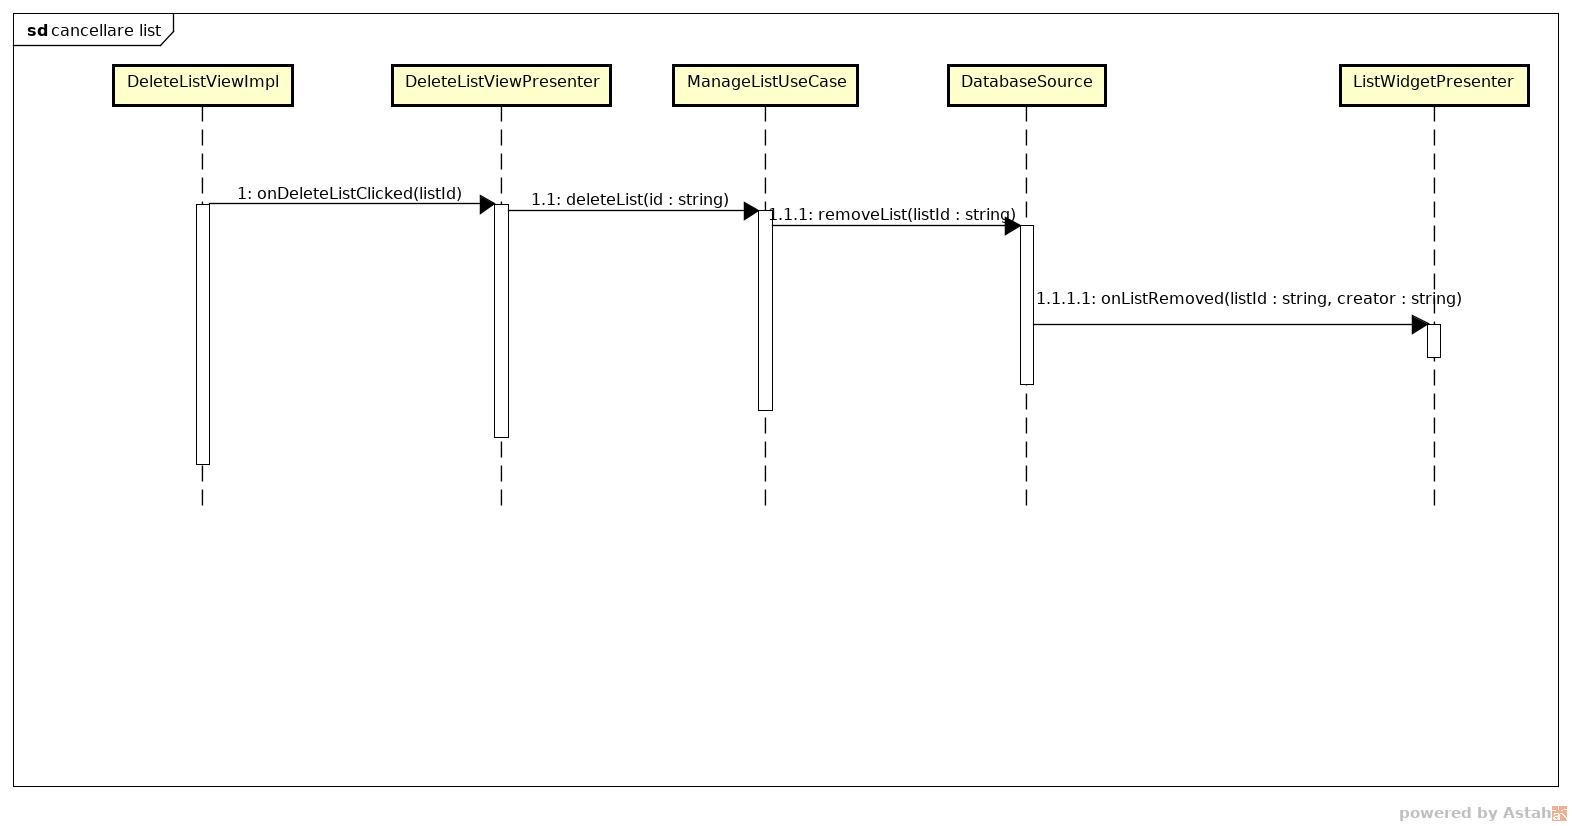
\includegraphics[width=\textwidth]{Sezioni/Diagrammi/img_app/cancellare_lista.jpg}
	\caption{Cancellazione di una lista}
\end{figure}

In questo scenario lo sviluppatore vuole cancellare la propria lista causando l'eliminazione da tutte le chat che la contengono. L'utente quando premerà il bottone elimina lista emetterà un evento che verrà successivamente catturato dalla classe \textit{deleteListViewImpl} che si occuperà di eliminare dal database la lista desiderata attraverso il suo \textit{presenter}. All'avvenuta eliminazione della lista nel \termine{database} verrà emesso l'evento che attiverà i metodi nel presenter della bolla lista per aggiornare, in questo caso eliminare definitivamente,tutte le chat contenti l'istanza di quella lista. 

\subsubsection{Modifica di una lista}

\label{Modifca di un lista}
\begin{figure}[H]
	\centering
	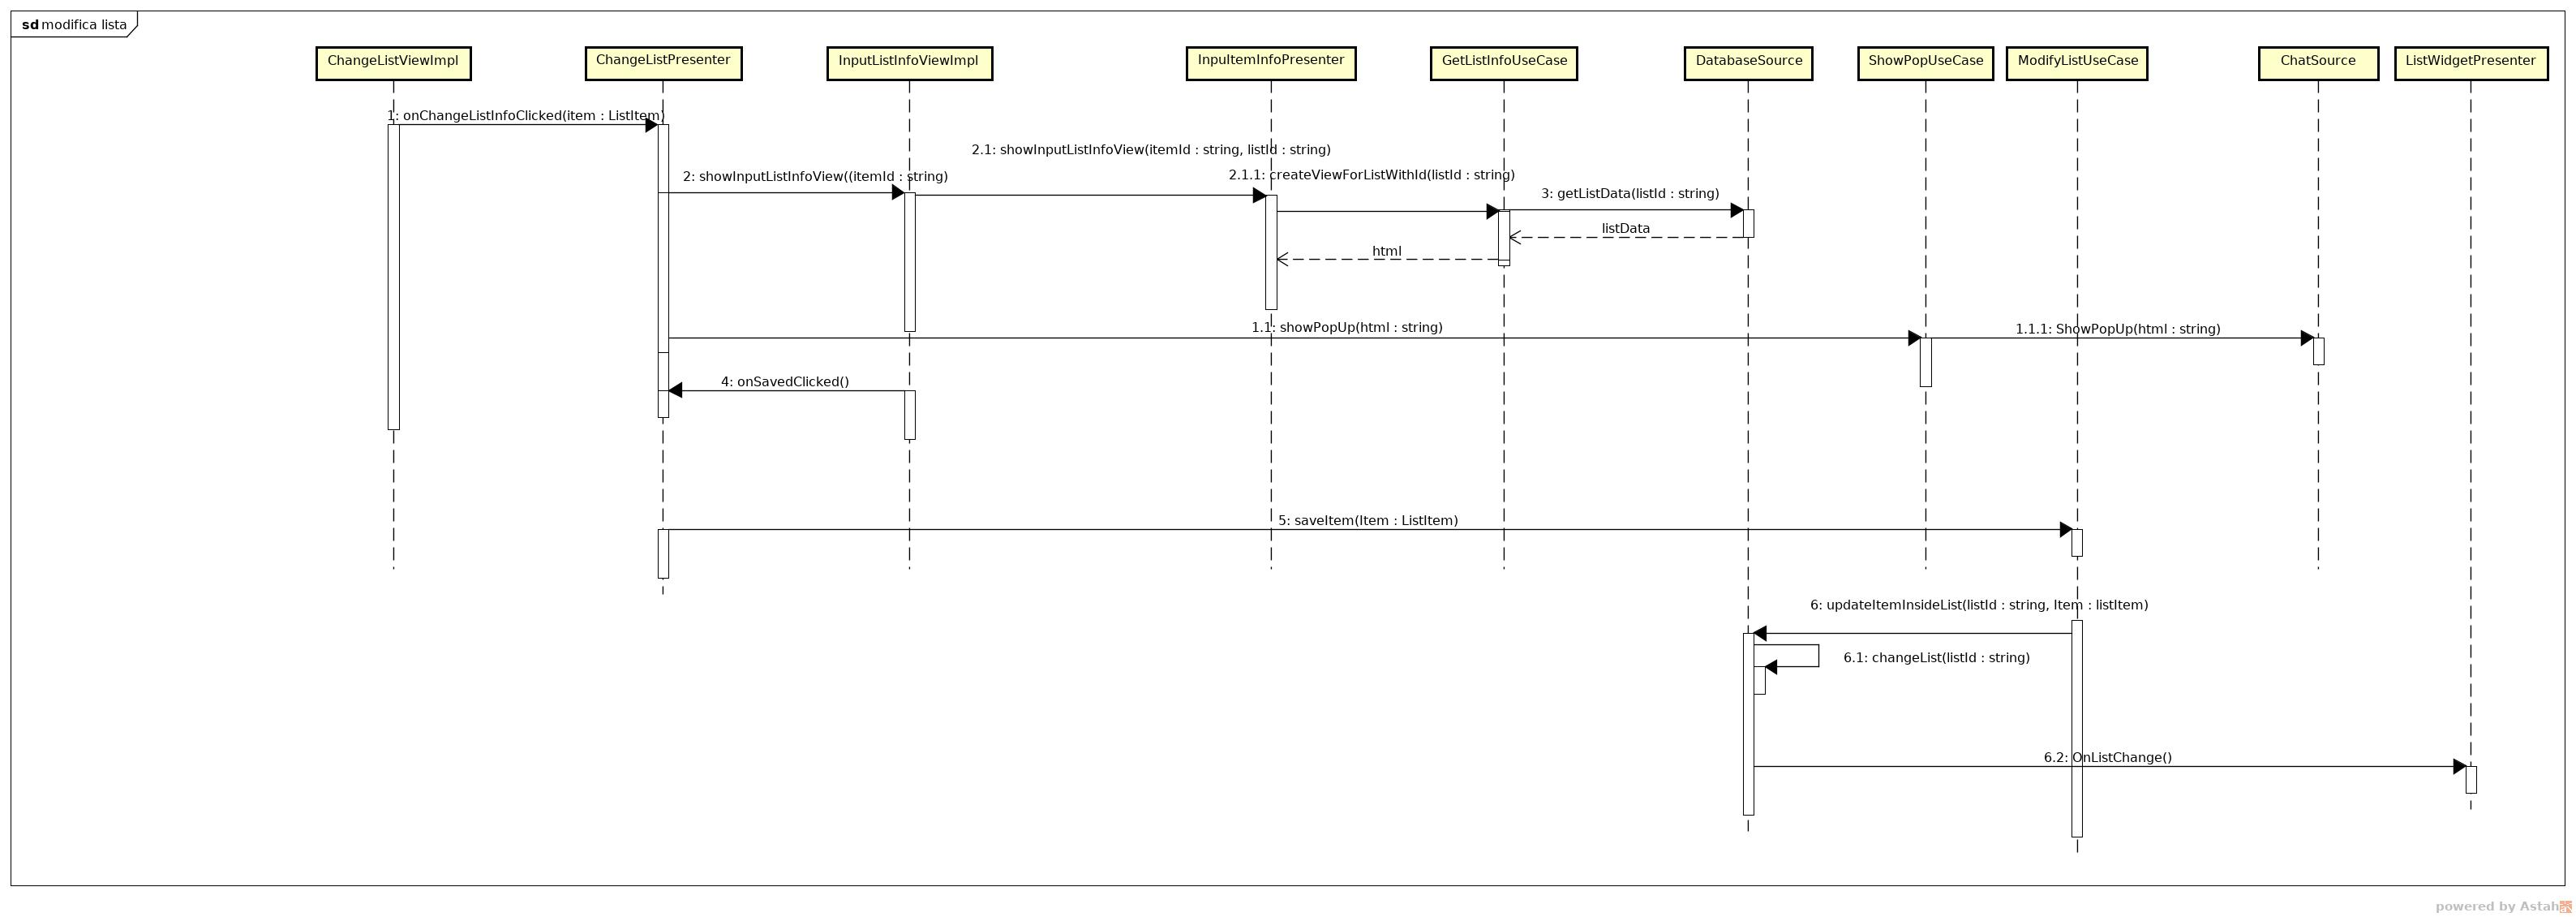
\includegraphics[width=\textwidth]{Sezioni/Diagrammi/img_app/modifica_lista.jpg}
	\caption{Modifica di una lista}
\end{figure}

In questo scenario lo sviluppatore vuole modifcare una lista cambiando, ad esempio, il suo nome o l'immagine ad essa associata. L'utente premendo il bottone modifica lista attiverà l'emissione di un evento che verrà catturato dalla classe \textit{ChangeListViewImpl} e demanderà la  gestione al suo presenter. Quest'ultimo attraverso il suo  metodo \textit{showInputListView} gli ritornerà l'html per la modifica della lista completa di tutte le informazioni di essa presenti nel \termine{database}. Successivamente richiamando il metodo \textit{showPopUp} si visualizzerà a schermo  le informazioni prima ottenute con la possibilità di modificarle. Una volta modificate le informazioni desiderate l'utente premerà il pulsante di conferma modifica in questo modo verrà emmesso l'evento di salvataggio che verrà catturato dalla classe \textit{InpuListInfoViewImpl} e successivamente demandato alla classe \textit{ChangeListPresenter} che si occuperà di salvare le modifiche nel \termine{database}.
All'avvenuta modifica della lista  verrà emesso l'evento che attiverà i metodi nel presenter della bolla lista per aggiornare tutte le chat contenti l'istanza di quella lista.
 
\subsubsection{Interazione con lista }

\label{Interaione con lista}
\begin{figure}[H]
	\centering
	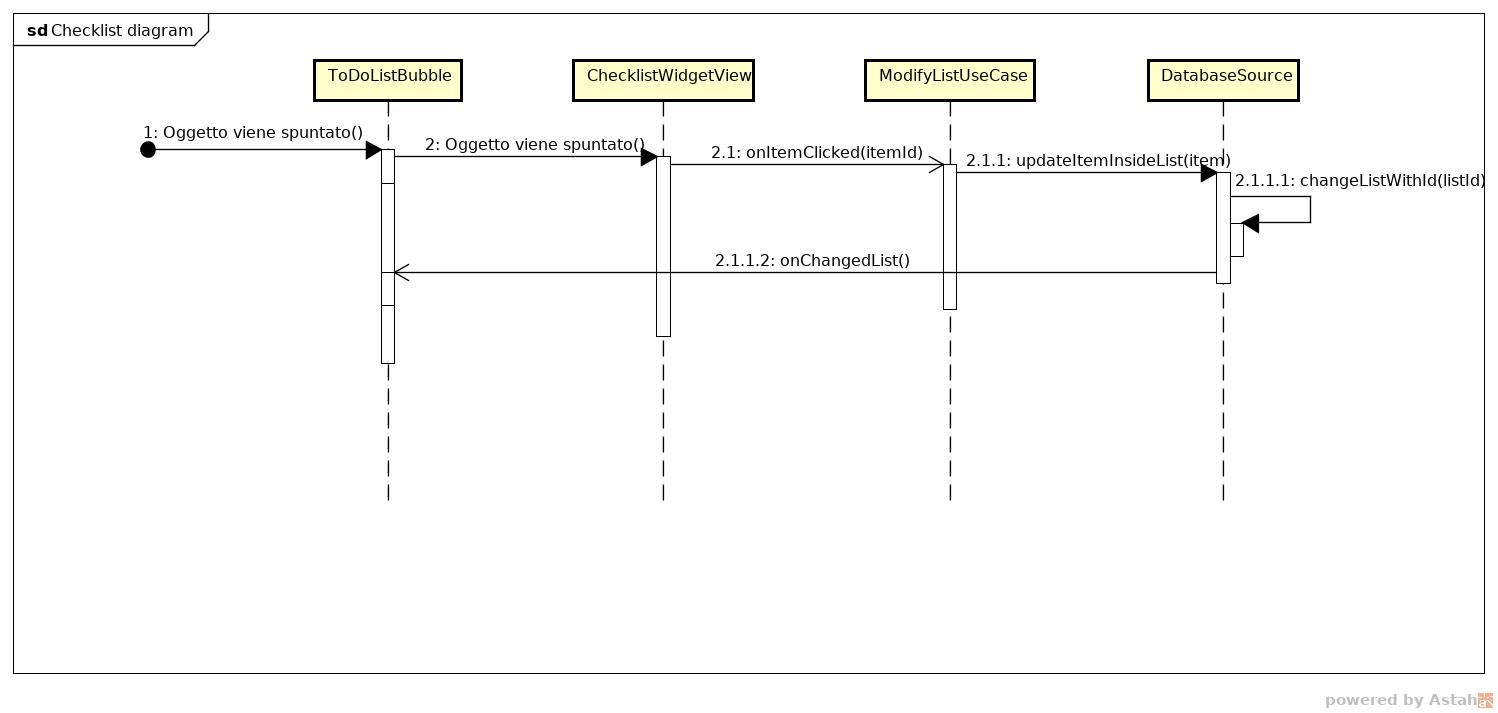
\includegraphics[width=\textwidth]{Sezioni/Diagrammi/img_app/Checklist_diagram.jpg}
	\caption{Interaione con lista}
\end{figure}

In questo scenario l'utente vuole spuntare un \termine{item} per segnarlo come \textit{acquistato}.
Per farlo l'utente clicca sul segno del quadrato, il click viene passato dalla bolla alla checklsit contenuta in essa, quindi viene emittato l'evento \textit{onItemClicked} identificando l'oggetto premuto. Ora lo usecase si occupa di aggiornare la lista chiamando il metodo \textit{updateItemInsideList} che chiama il metodo changeList di DatabaseSource per aggiornare la lista memorizzata. Una volta aggiornata, viene lanciato l'evento onChangedList che comunica l'avvenuto cambiamento.


\subsubsection{Aggiunta di un Item}

\label{Aggiunta di un Item}
\begin{figure}[H]
	\centering
	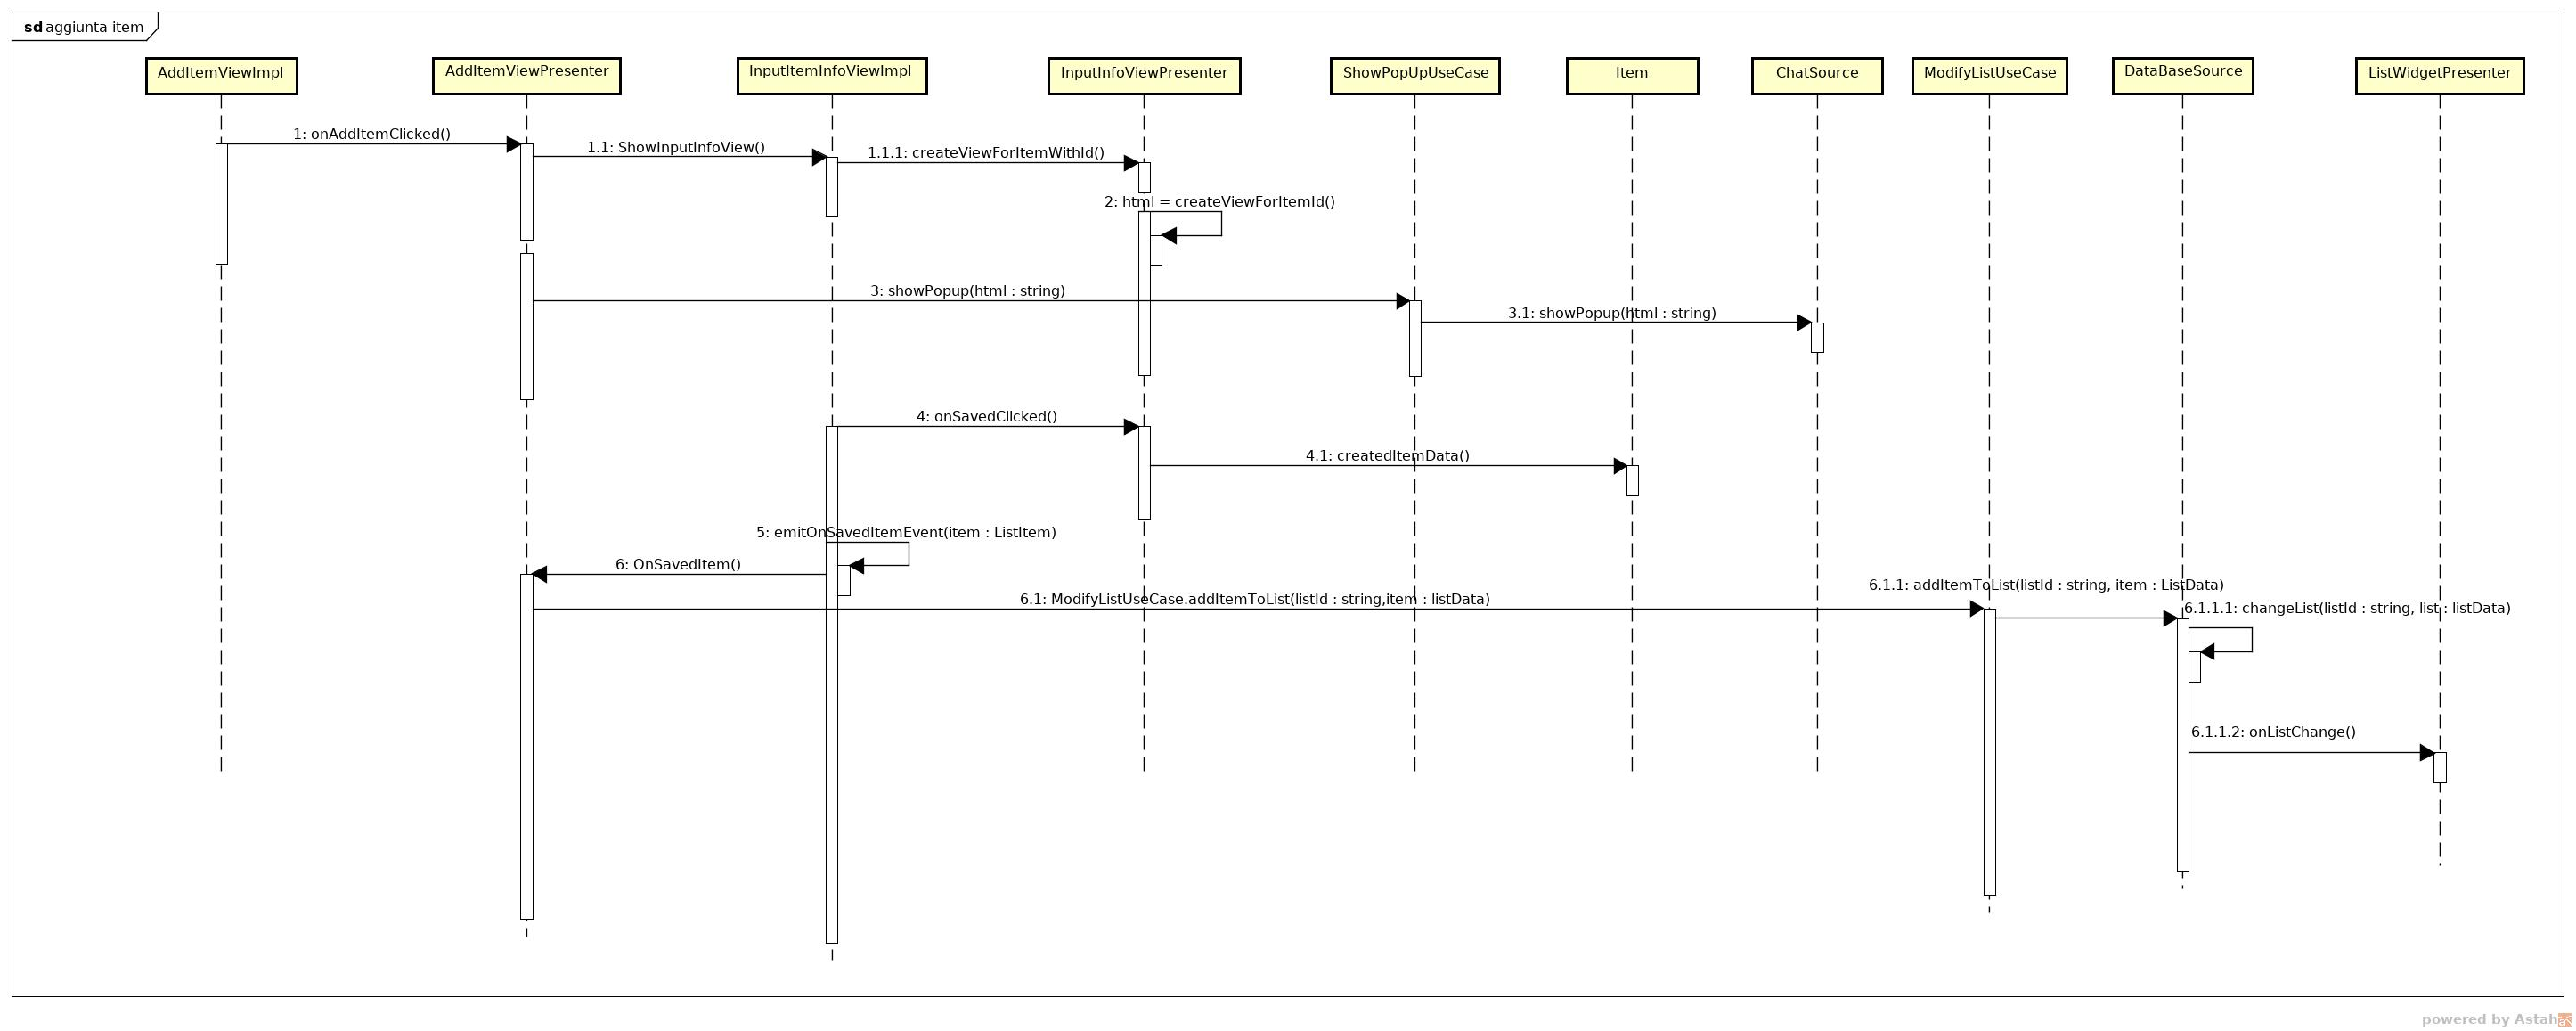
\includegraphics[width=\textwidth]{Sezioni/Diagrammi/img_app/aggiunta_item.jpg}
	\caption{Aggiunta di un Item}
\end{figure}

In questo scenario lo sviluppatore vuole aggiungere dei prodotti (chiamati \termine{item} nella nostra applicazione) alla lista da esso creata. Oppure vuole aggiungerli a una lista nella quale ha permessi di modifca. L'utente premendo il pulsante \textit{aggiungi item} farà emettere un evento che verrà catturato dalla classe \textit{AddItemViewImpl} che demanderà la gestione al suo presenter. Quest'ultimo attraverso il metodo \textit{showInputInfoView} recupererà l'html necessario per la corretta aggiunta di un item e successivamente attraverso la classe \textit{showPopUpUseCase} farà visualizzare a schermo le informazioni prima recuperate. L'utente una volta che ha inserito le informazioni desiderate premerà il pulsante di aggiunta del item. In questo modo verrà emesso l'evento di salvataggio che verrà poi catturato dalla classe \textit{InputItemInfoViewImpl} che si occuperà di creare l'item ed emettere un evento per l'avvenuta creazione ed infine la classe \textit{AddItemViewPresenter} si occuperà di memorizzare la  lista con il nuovo \termine{item} nel \termine{database}. Infine all'avvenuta modifca della lista nel \termine{database} verrano eseguiti i metodi nel presenter della bolla lista per aggiornare tutti le chat contenenti l'istanza della lista appena modificata. 




\subsubsection{Modifica Item}

\label{Modifica Item}
\begin{figure}[H]
	\centering
	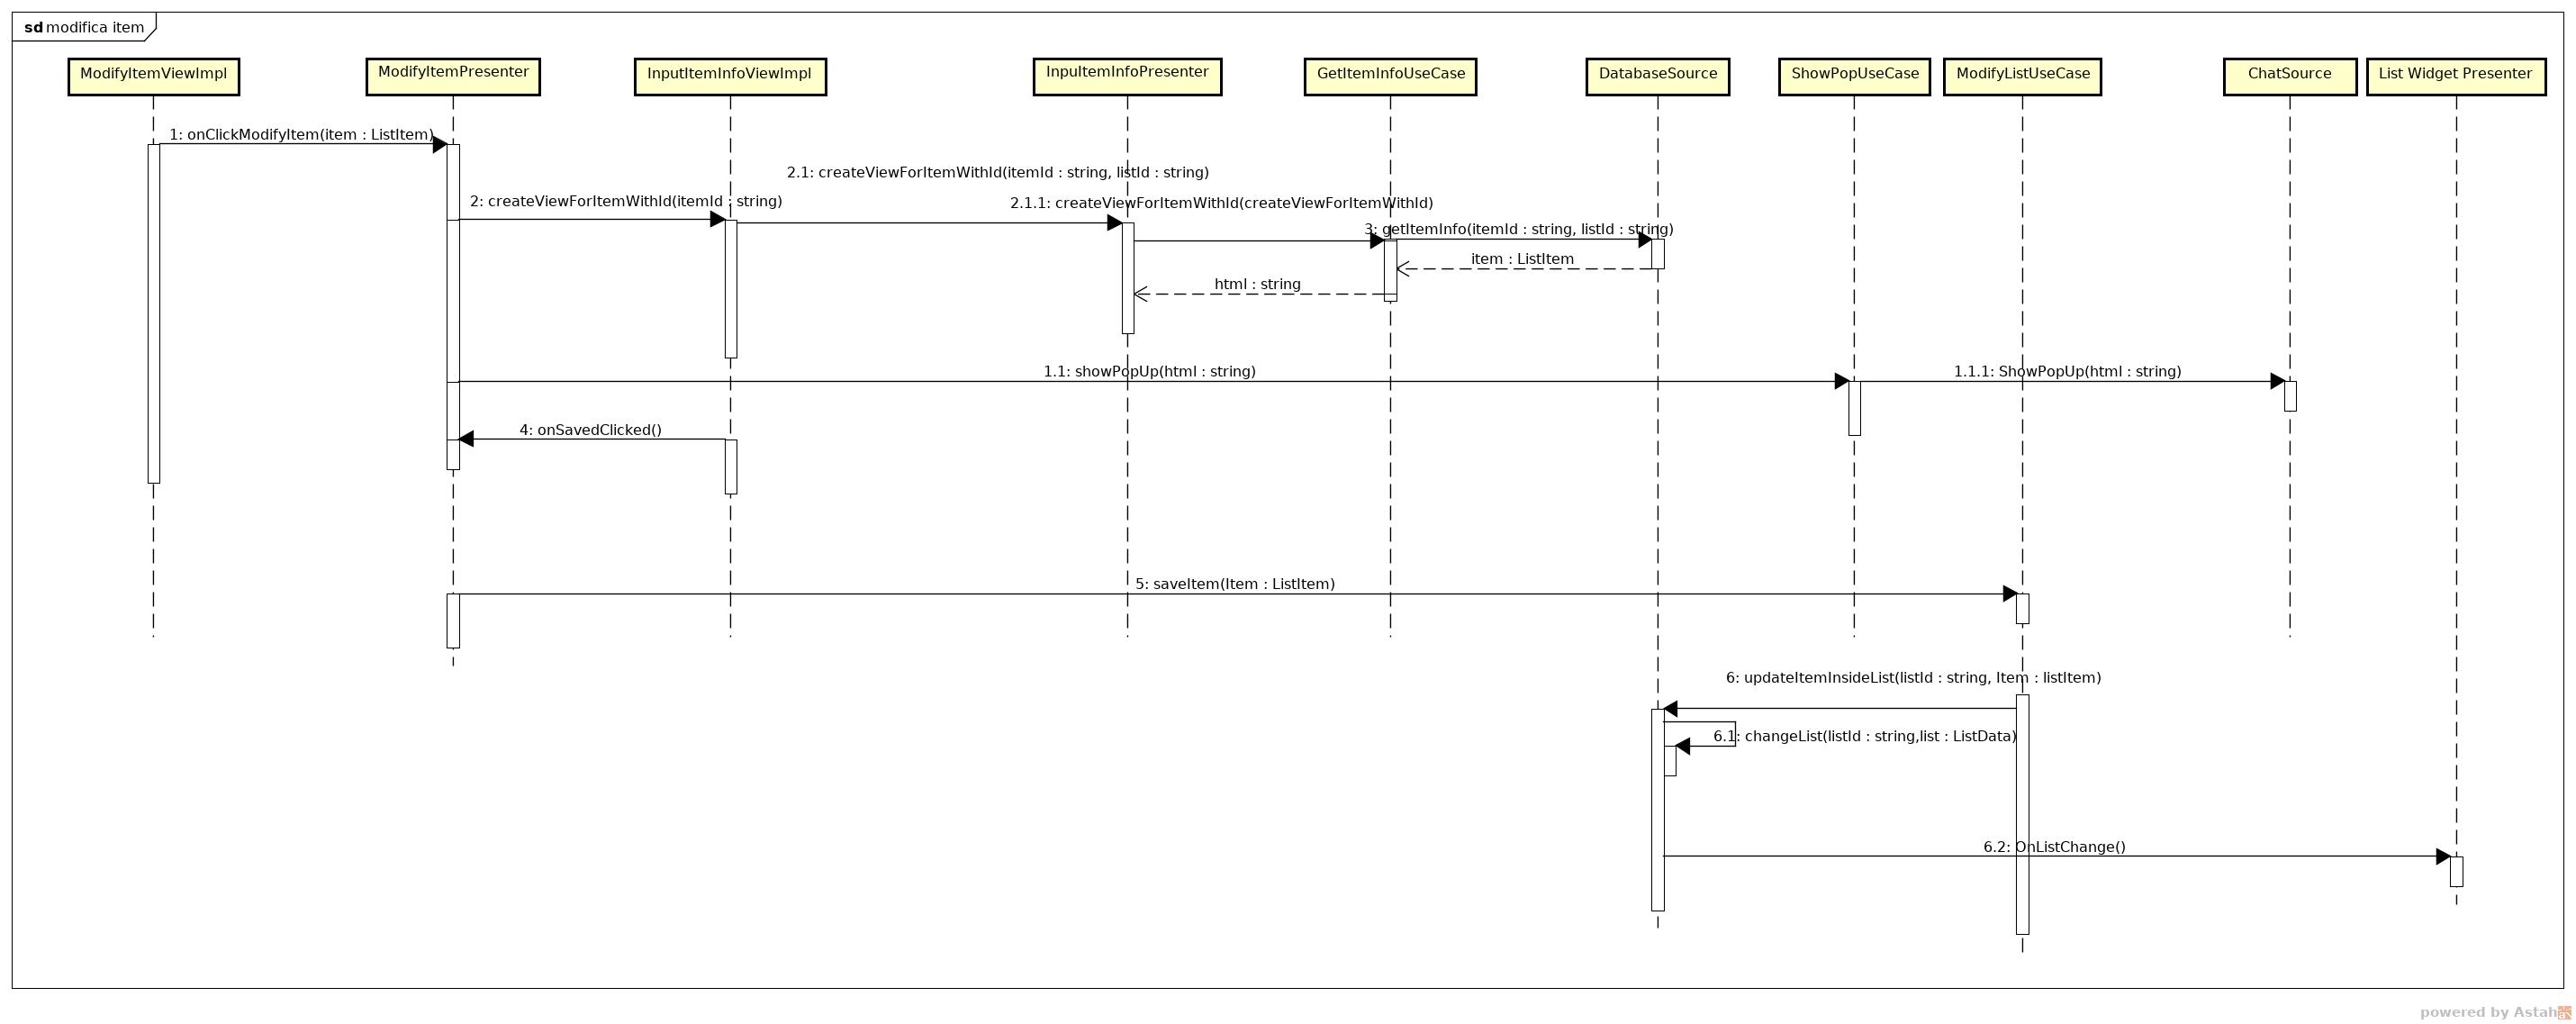
\includegraphics[width=\textwidth]{Sezioni/Diagrammi/img_app/modifica_item.jpg}
	\caption{Modifica Item}
\end{figure}

In questo scenario lo sviluppatore vuole modificare le informazioni di un \termine{Item} già presente nella lista. L'utente premendo il bottone per la modifca di un item attiverà l'emissione di un evento che verrà catturato dalla classe \textit{ModifyItemViewImpl} demandando la gestione al suo presenter. Quest'ultimo attraverso il suo metodo \textit{createViewForItemWithId} gli ritornerà l'html per la modifica del \termine{item} completo di tutte le informazioni di esso, presenti nel \termine{database}. Successivamente richiamando il metodo \textit{showPopUp} l'utente visualizzerà a schermo le informazioni prima ottenute con la possibilità di mofica. Una volta modificate le informazioni desiderate l'utente premerà il pulsante di conferma modifica, verrà quindi emesso l'evento di salvataggio che verrà catturato dalla classe \textit{InputItemInfoViewImpl} e successivamente demandato a \textit{ModifyItemPresenter} che si occuperà di salvare le modifiche effettuate nel \termine{database}. Infine all'avvenuta modifca della lista nel \termine{database} verrano eseguiti i metodi nel presenter della bolla lista per aggiornare tutti le chat contenenti l'istanza della lista appena modificata. 

\subsubsection{Rimozione Item}

\label{Rimozione Item }
\begin{figure}[H]
	\centering
	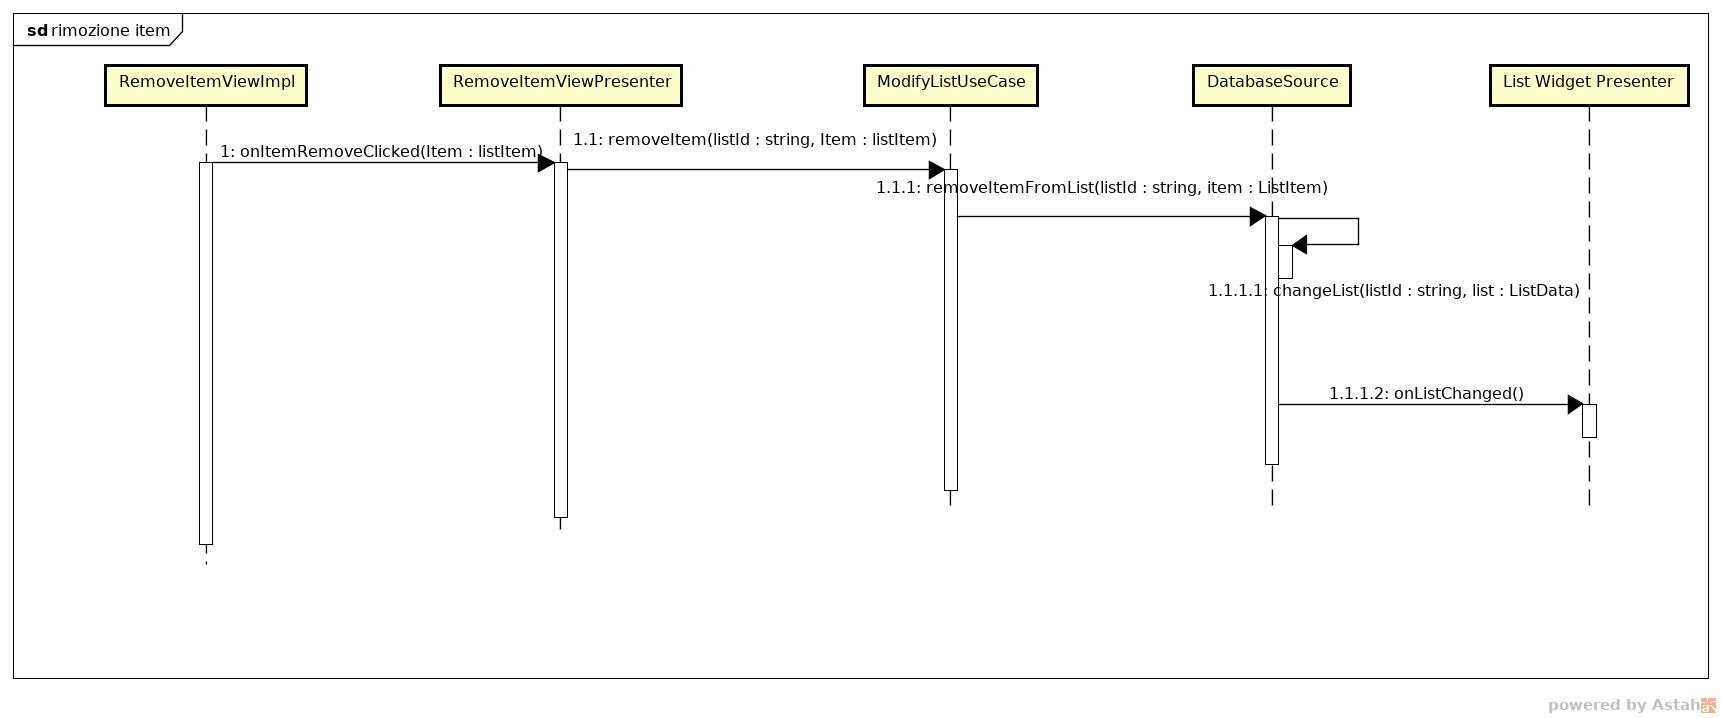
\includegraphics[width=\textwidth]{Sezioni/Diagrammi/img_app/rimozione_item.jpg}
	\caption{Rimozione Item}
	
\end{figure}
In questo scenario l'utente vuole eliminare un item dalla lista. Per farlo l'utente deve premere il pulsante rimuovi item attivando quindi un evento che verrà catturato dalla classe \textit{RemoveItemViewImpl} demandando la gestione al suo presenter. Quest'ultimo attraverso il metodo \textit{removeItem} eliminerà l'item della lista corrente nel \termine{database}.Infine all'avvenuta modifca della lista nel \termine{database} verrano eseguiti i metodi nel presenter della bolla lista per aggiornare tutti le chat contenenti l'istanza della lista appena modificata.  
\newpage

\subsubsection{Pubblicazione a un contatto}

\label{Pubblicazione di un contatto}
\begin{figure}[H]
	\centering
	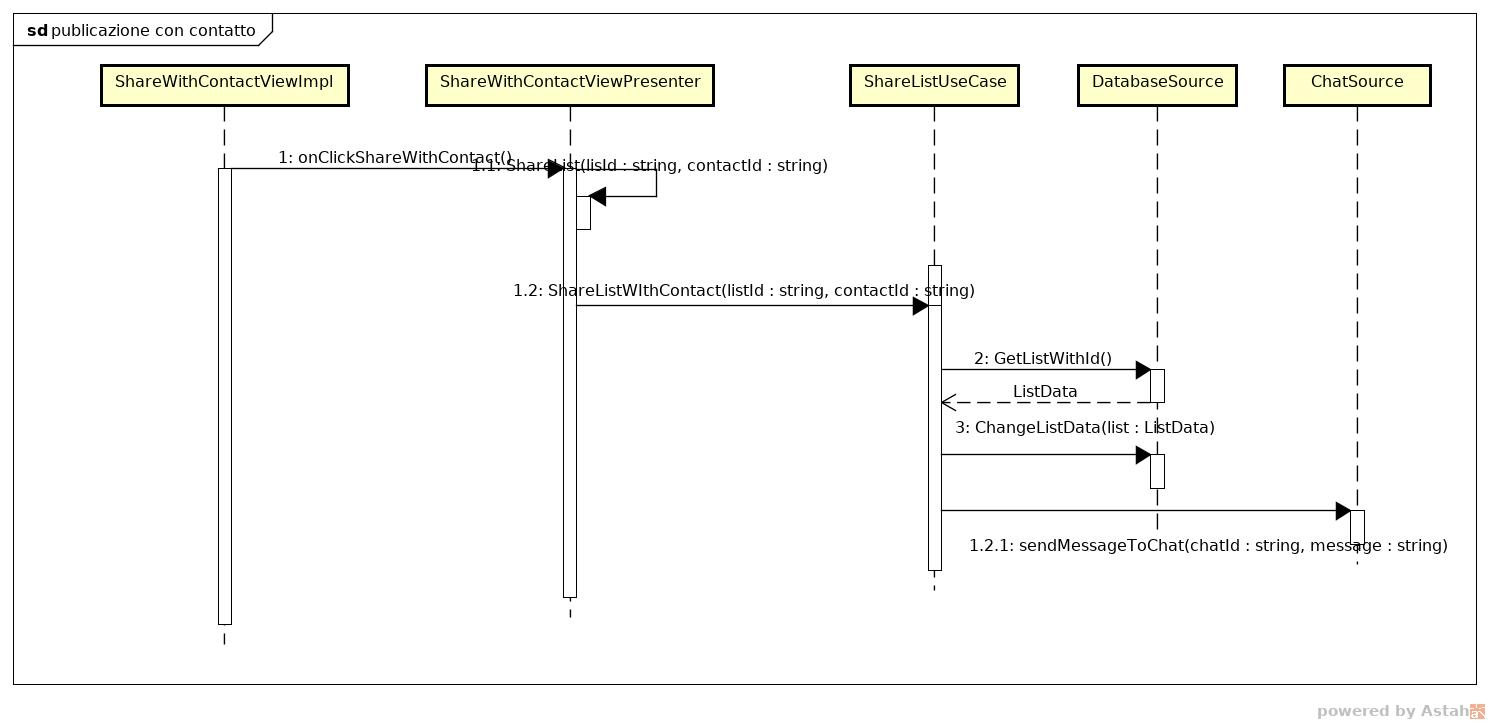
\includegraphics[width=\textwidth]{Sezioni/Diagrammi/img_app/publicazione_con_contatto.jpg}
	\caption{Pubblicazione di un contatto}
	
\end{figure}
In questo scenario l'utente vuole pubblicare la lista a un altro contatto, dando il permesso di modifica e interazione con la lista. L'utente premendo il bottone \textit{pubblica lista} sceglierà un contatto, lanciando quindi un evento che verrà catturato dalla classe \textit{ShareWithContactViewImpl} e demandato al suo presenter che tramite il metodo \textit{shareList} attiverà i metodi utili per aggiungere i permessi necessari al interazione al utente scelto. Successivamente la classe \textit{ShareListUseCase} si occuperà di salvare le modifiche nel \termine{database} e pubblicare infine al utente desiderato la lista tramite il metodo {sendMessageToChat}.


\subsubsection{Pubblicazione a un gruppo}

\label{Pubblicazione a un gruppo}
\begin{figure}[H]
	\centering
	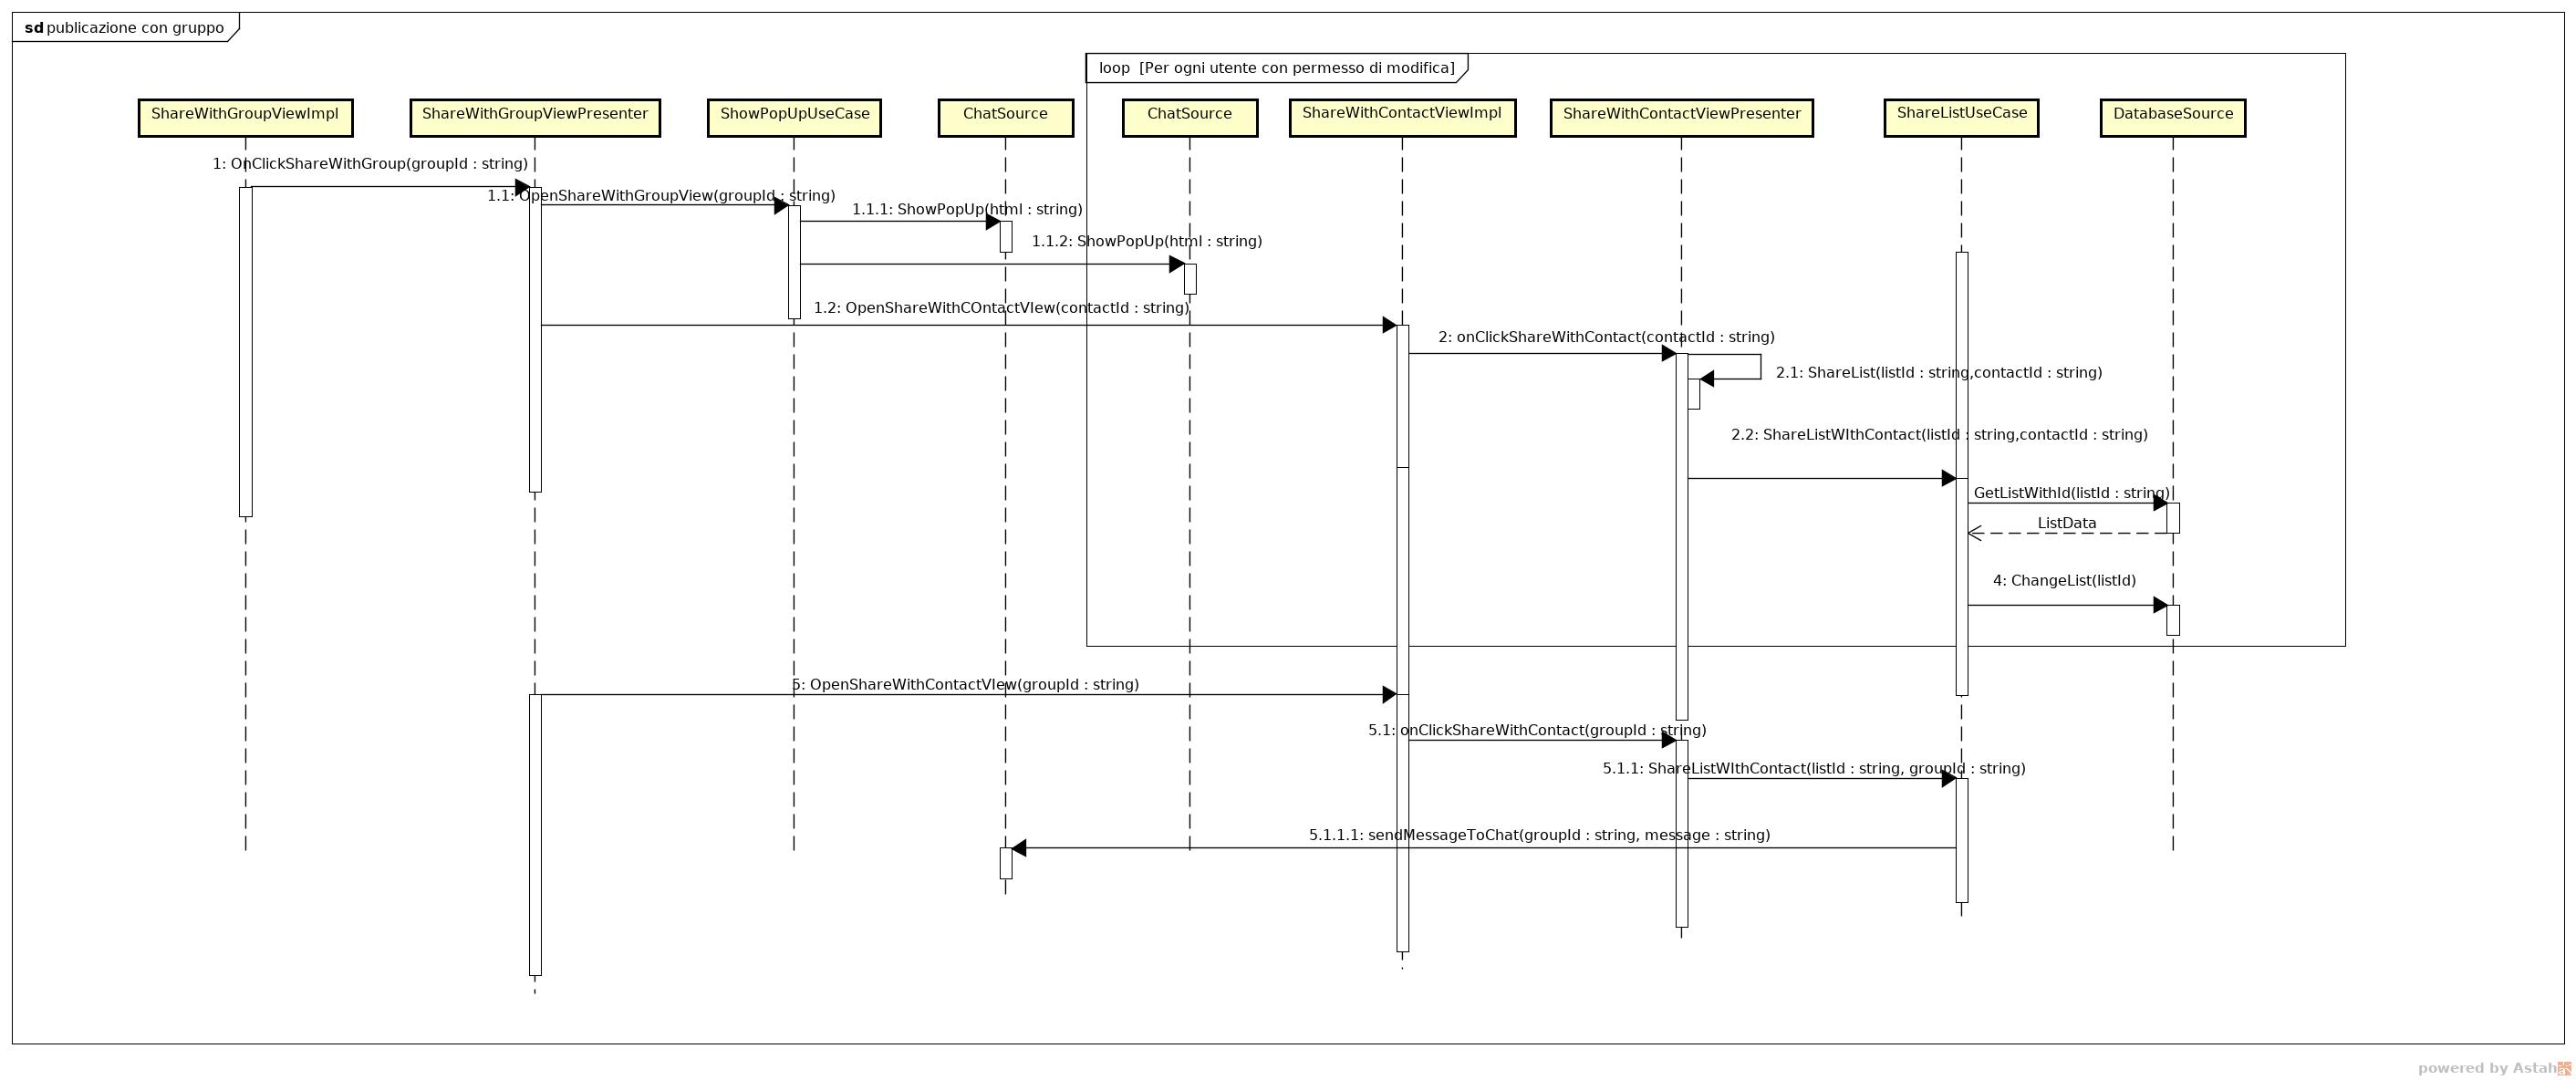
\includegraphics[width=\textwidth]{Sezioni/Diagrammi/img_app/publicazione_con_gruppo.jpg}
	\caption{Pubblicazione a un gruppo}
	
\end{figure}

Simile allo scenario precedente in questo caso l'utente vuole condividere e dare i permessi ad utenti speicifici presenti nel gruppo. L'utente premendo il bottone \textit{pubblica lista} sceglierà un gruppo, lanciando quindi un evento che verrà catturato dalla classe \textit{ShareWithGroupViewImpl}
\newpage e demenderà la gestione al suo presenter. Quest'ultimo attraverso il metodo OpenShareWithGroup inizializzerà un ciclo che porterà a scegliere per ogni utente presente nel gruppo la negazione o meno dei permessi. La procedura per svogere il ruolo sopradescritto è simile allo scenario della \textit{pubblicazione con contatto} con la differenza che non verrà inviato un messaggio agli utenti con i permessi concessi. Infine terminato il ciclo verrà pubblicata la lista nel gruppo attraverso il metodo \textit{openShareWithContactView} nel quale passera come parametro di ingresso l'id del gruppo; che invierà il messaggio nel gruppo desiderato.

\subsubsection{Inoltro a un contatto}

\label{Inoltro a un contatto}
\begin{figure}[H]
	\centering
	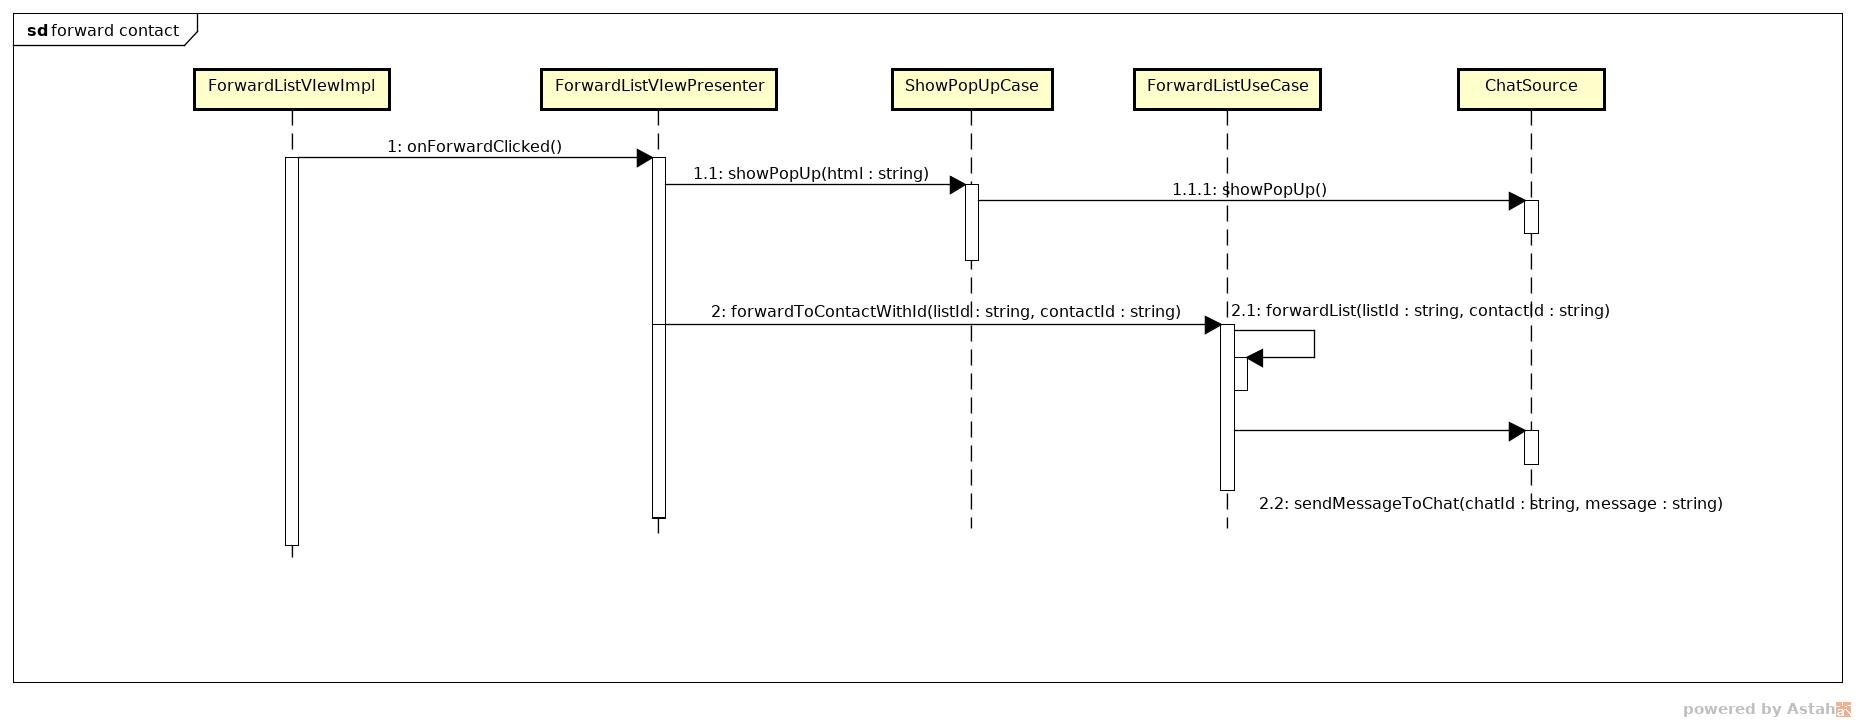
\includegraphics[width=\textwidth]{Sezioni/Diagrammi/img_app/forward_contatto.jpg}
	\caption{Inoltro a un contatto}
	
\end{figure}

In questo scenario l'utente vuole inoltrare la lista a un contatto come fosse un semplice messaggio di testo, senza aggiungere al specifico contatto nessun permesso di modifica o interazione. L'utente premendo il bottone di inoltro sceglie un contatto. Si verifica quindi l'evento che verrà catturato dalla classe \textit{ForwardListViewImpl} demandandone la gestione al suo presenter.
Quest'ultimo con il metodo \textit{forwardToContactWithId} inoltrerà la lista al contatto desiderato attraverso la classe \textit{ChatSource}.Prima del avvenuto inoltro al contatto selezionato è presente il metodo \textit{showPopUp} che interfaciandosi con la classe \textit{ForwardListUseCase} mostrerà a schermo un messaggio di conferma per l'inoltro e la scelta per il contatto a cui inoltrare il messaggio.



\subsubsection{Inoltro a un gruppo}

\label{Inoltro a un contatto}
\begin{figure}[H]
	\centering
	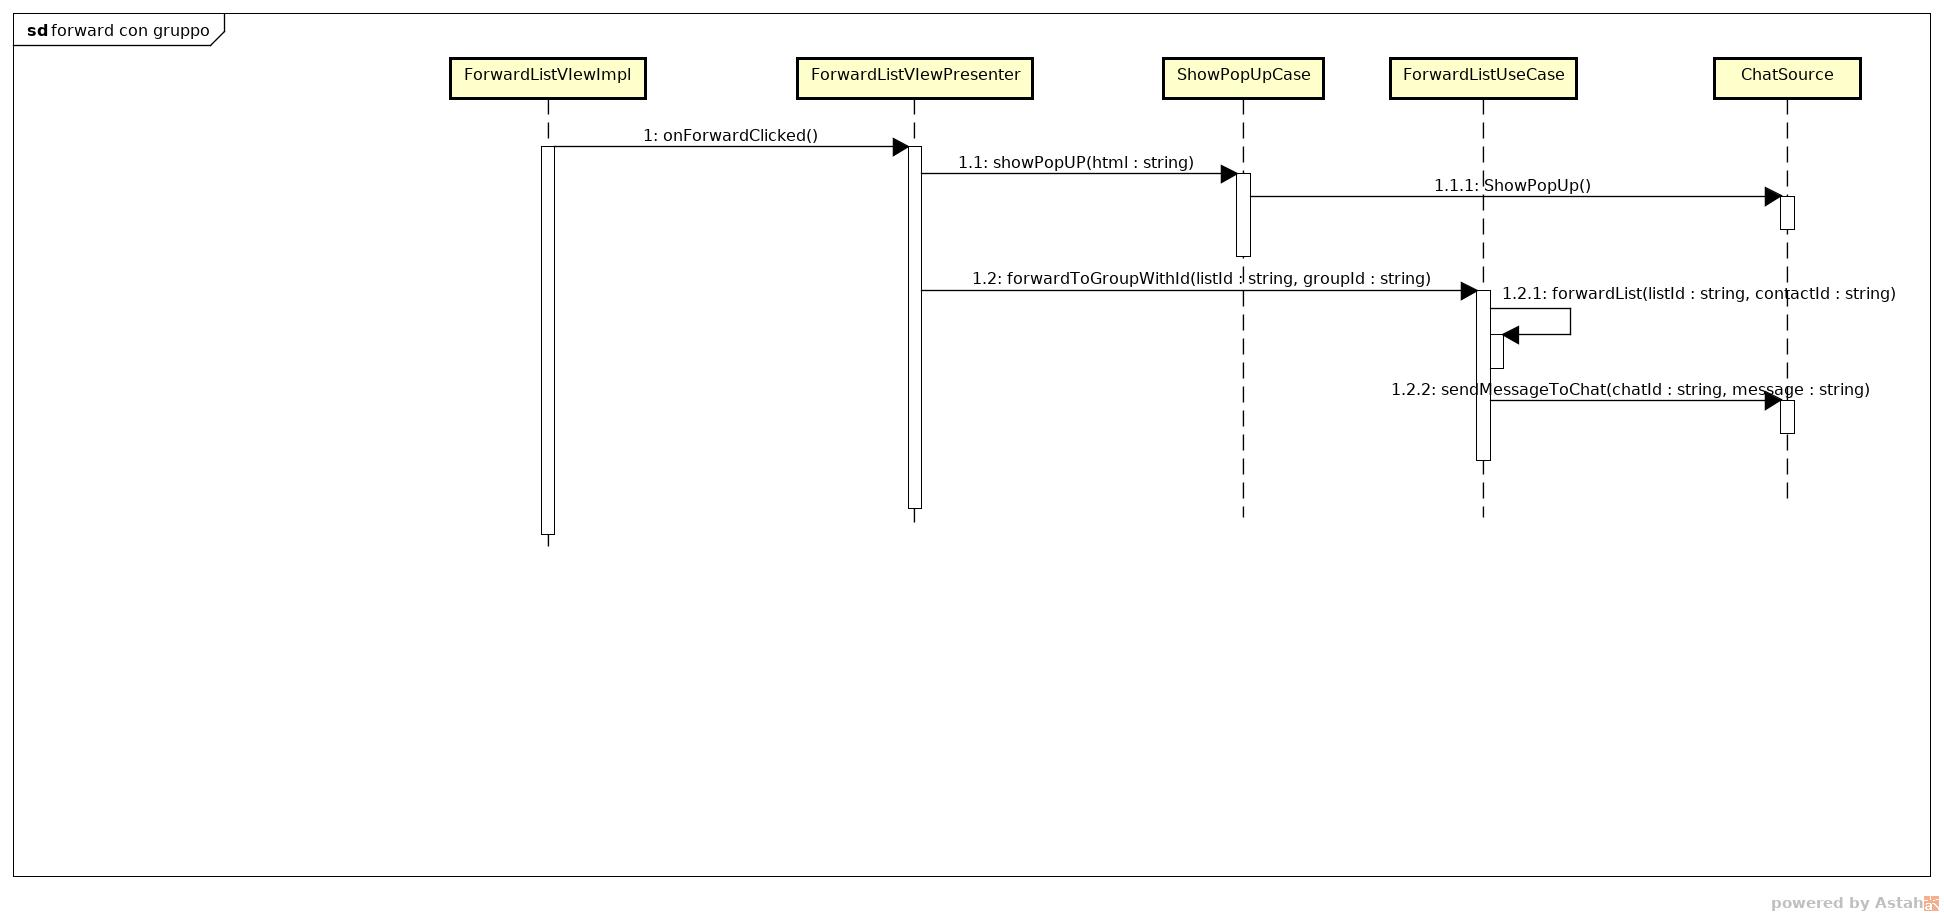
\includegraphics[width=\textwidth]{Sezioni/Diagrammi/img_app/forward_con_gruppo.jpg}
	\caption{Inoltro a un contatto}
	
\end{figure}

In questo scenario l'utente vuole inoltrare la lista a un gruppo come fosse un semplice messaggio di testo, senza aggiungere al specifico gruppo nessun permesso di modifica o interazione. L'utente premendo il bottone di inoltro sceglie un gruppo. Si verifica quindi l'evento che verrà catturato dalla classe \textit{ForwardListViewImpl} demandandone la gestione al suo presenter.
Quest'ultimo con il metodo \textit{forwardToGroupWithId} inoltrerà la lista al gruppo desiderato attraverso la classe \textit{ChatSource}.Prima del avvenuto inoltro al gruppo è presente il metodo \textit{showPopUp} che interfaciandosi con la classe \textit{ForwardListUseCase} mostrerà a schermo un messaggio di conferma per l'inoltro e la selezione del gruppo a cui si desidera inoltrare.


\subsubsection{Help}

\label{Help}
\begin{figure}[H]
	\centering
	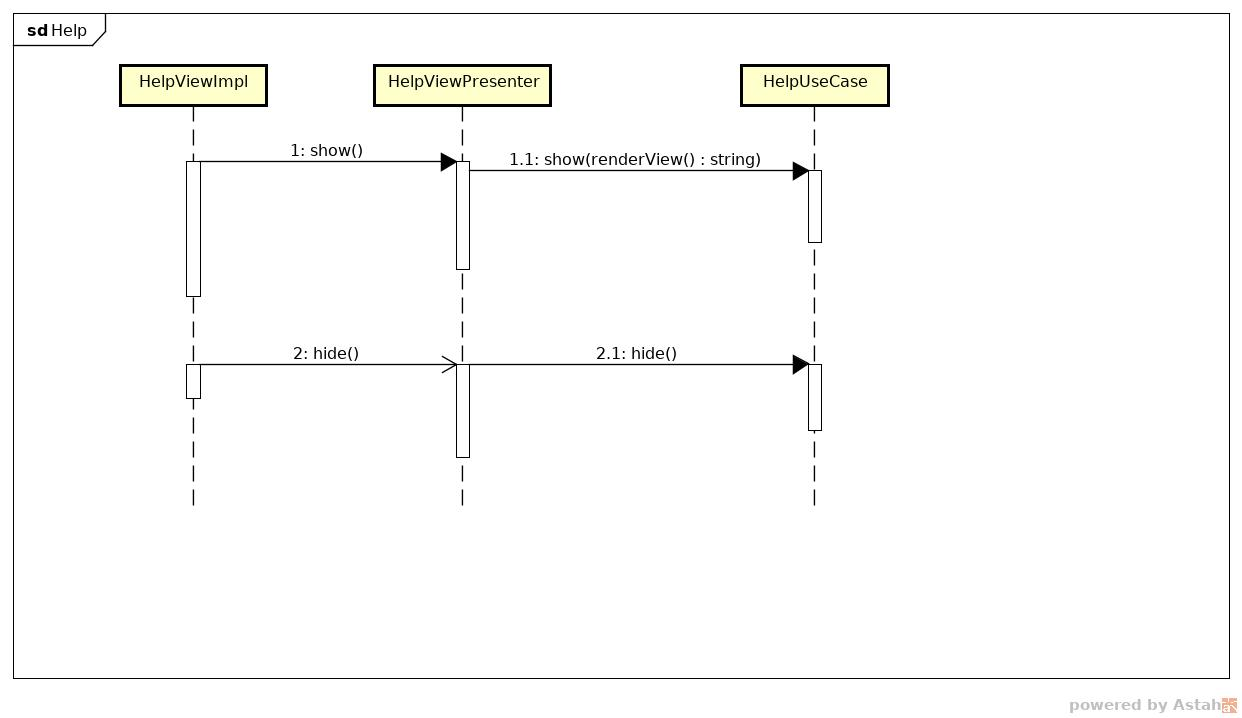
\includegraphics[width=\textwidth]{Sezioni/Diagrammi/img_app/Help.jpg}
	\caption{Help}
	
\end{figure}

In questo scenario l'utente vuole chiedere delle informazioni d'aiuto per l'utilizzo della nostra appliazione. Per richiedere aiuto l'utente può schiacciare il bottone di help apposito. In questa maniera viene attivato un metodo nella classe \textit{HelpViewImpl} che demandanderà la gestione al suo presenter. Quest'ultimo attraverso il metodo \textit{show} farà visualizzare a schermo un popup con le informazioni utili. Per nascondere le informazioni d'aiuto avremo lo stesso flusso di utilizzo con il metodo \textit{hide} in sostituzione al metodo \textit{show} attivabile nella stessa maniera.
